\documentclass{sig-alternate}
\usepackage{color}
\usepackage[colorinlistoftodos]{todonotes}
\usepackage{graphicx}
\graphicspath{ {images/} }
\usepackage{mathtools}
\usepackage{amsmath}

\begin{document}
\conferenceinfo{UMM CSci Senior Seminar Conference, December 2015}{Morris, MN}

\title{Thermal Interaction In Spatial Augmented Reality}

\numberofauthors{1}

\author{
% The command \alignauthor (no curly braces needed) should
% precede each author name, affiliation/snail-mail address and
% e-mail address. Additionally, tag each line of
% affiliation/address with \affaddr, and tag the
% e-mail address with \email.
\alignauthor
Justin B. YaDeau\\
	\affaddr{Division of Science and Mathematics}\\
	\affaddr{University of Minnesota, Morris}\\
	\affaddr{Morris, Minnesota, USA 56267}\\
	\email{yadea003@morris.umn.edu}
}

\maketitle

\begin{abstract}
I will discuss two approaches in this paper; one approach goes over the use of thermal sensors to be able to utilize most surfaces with mobile technology. The other approach uses spatial augmented reality as a tool for 3D data visualization. Taking both of these ideas and putting them together is the goal of this paper. A phone having the ability to know exactly where a user put their finger, and correlate that to a program or some other process, would be helpful in advancing the use of smaller mobile technology. Also, being able to interact with charts, maps, or graphs without having to actually touch an electronic device. This can reduce the amount of electronic devices needed for modern life. I will discuss both studies and then join them together in a way to minimizes the limitations that each has. Showing the possible applications that would be possible when joining these two methods and how they benefit us.

\end{abstract}

\keywords{thermal interaction, 3D data visualization, augmented reality, AR, spatial augmented reality, SAR}

\section{Introduction}
\label{sec:Introduction}
Imagine being able to touch a table and have a phone know the location of the interaction. Now think of the same scenario, but this time the phone says the number 0 was pressed because the area touched corresponded to the number 0 on a dial pad that your phone thinks is on the surface. Research by Kurz \cite{Thermal} addresses this topic, being able to use thermal technology to accurately tell if a surface was touched by a finger and where. Kurz \cite{Thermal} states that as wearable technology becomes more prominent, alternative solutions to touch screens will be sought after. With that in mind being able to interact with technology with a screen would help advance the wearable technology.    

Now think of a table that has a cone on it with projectors displaying data on the cone. This is how Thomas et al. describes one of the ways to utilized spatial augmented reality as a tool for 3D data visualization. Using technologies to track where the user is and being able to move the cone to define a new visualization. Also mentioning the scalability of the proposed system. CAVE systems would be the larger versions of the table-top design mentioned above.      

I will discuss both studies and then join them together in a way to minimizes the limitations that each has. Showing the possible applications that would be possible when joining these two methods.       


\section{Background}
\label{sec:background} 
Before starting this paper there are some concepts that should be made clear. It will be helpful to have a clear understanding of the differences between virtual reality, augmented reality, and spatial augmented reality. Also knowing the concept of six degrees of freedom is beneficial.  

\subsection{Virtual Reality}
\label{sec:Virtual Reality}
In my personal opinion, one of the more well known example of Virtual Reality (VR) today is the Oculus Rift. An earlier take on this type of VR from Nintendo in the 90's is the Virtual Boy. Like the Oculus Rift the Virtual Boy is a device that strapped to the head of the user and used to simulate a virtual world mainly though sight. As you turn your head, the field of view in the virtual world will change accordingly. An earlier example would be the view master, the stereoscopic toy that had circular inserts requiring the user to look into a light source to illuminate the picture. Being more primitive, the view masters creates a visual sensory experience. Other VR systems ``artificially creates sensory experiences, which can include sight, hearing, touch, and smell'' \cite{VR}. The most common experiences that VR creates for a user is sight and sound.       

\subsection{Augmented Reality}
\label{sec:Augmented Reality}
Augmented Reality (AR) can be described as augmenting the environment of the real world. It's different from VR because it is based in the physical world instead of the digital world. An example is Google Translate: using the camera from a phone, it translates foreign word(s) that the camera is pointed at. Using a program it can detect words from most languages, this works best with printed text. Then the program overlays the translation onto the sign, billboard, or menu on the screen, using the same font and font size as the original text. Another example would be for anyone who bought a 3DS might know the 3D cards the system came with, those are also a form of AR. A 3DS is a hand held gaming device that make the game being played 3D without the use of 3D glasses. The cards that came with the system were little mini games. Placing a card on the table, or any surface, and going into the application started a game. Creatures would pop up that the user would fight, or trying to hit bulls-eye on target. All this is done on the surface the card was placed on.   

\subsection{Spatial Augmented Reality}
\label{sec:Spatial Augmented Reality}
Spatial Augmented Reality (SAR) is similar to AR. The difference is that it focuses more on augmenting reality through projection technology, instead of using conventional monitors or other such devices. A good example of SAR is if a user has a sandbox with a topographical map overlaid onto the sand. They could move the sand around and the projector would be able to detect the height of the sand and match the peaks and valleys in the sand with the correct topographic overlay for displaying peaks and valleys. The way Thomas et al \cite{3D} defines SAR is 
\begin{quote}
Spatial Augmented Reality (SAR) enhances the visual aspects of physical objects, allowing users to better understand the virtual content. The users not only view the digital information but also gain a tactile understanding through touching the physical object.
\end{quote}

\subsection{6DOF}
\label{sec:6DOF}
6DOF, 6 degrees of freedom, are the different ways one can move in three dimensional space. Front/back, left/right, up/down, roll, pitch, yaw are all the ways to move in 3D space. Roll is moving clockwise or counter clockwise in relation to the front/back axis. Yaw is moving the front/back axis to either left/right axis. Pitch is the same yaw, except the up/down axis instead of the left/right axis. For clarification see Figure \ref{fig:6DOF}

\begin{figure}
	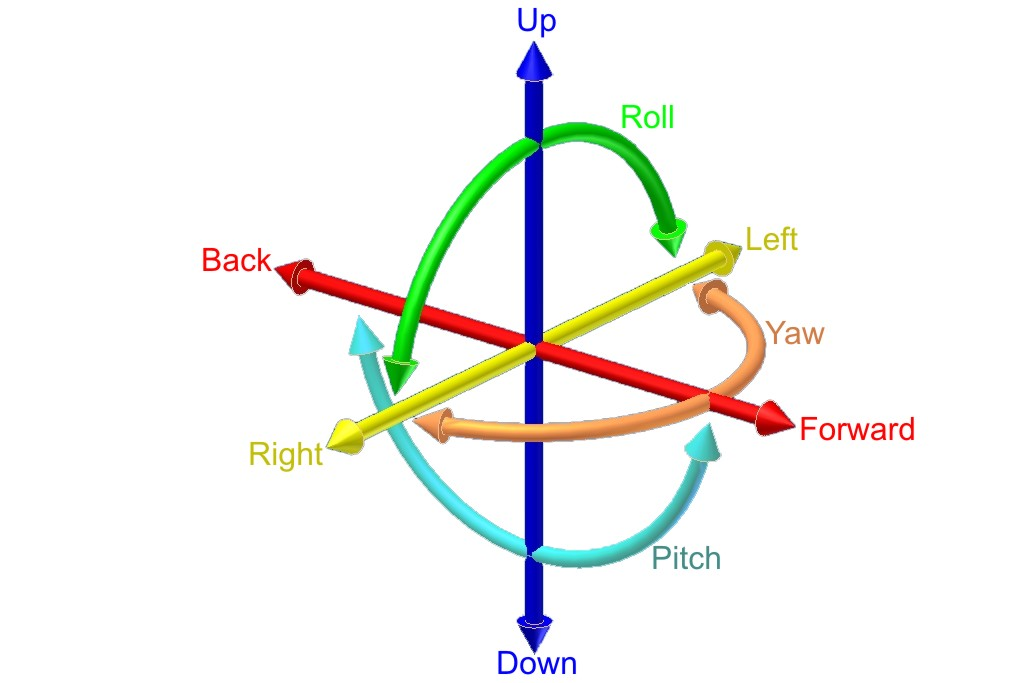
\includegraphics[width=8.5cm, height=5cm]{6DOF_en}
	\caption{6DOF axises related to 3D space \cite{6DOF}}
	\label{fig:6DOF}
\end{figure}  


\section{Thermal Interaction}
\label{sec:Thermal Interaction}
Kurz \cite{Thermal} provides a way to interact with AR applications using almost any surfaces. Using infrared thermography, his system can detect if the user touched a surface or came close to touching it. Keeping in mind that one's finger(s) are warm and the surface is presumably cool, a touch leaves a heat signature on the cool surface. Kurz's system assumes that the interaction is taking place in a controlled environment where surfaces will be cooler than body temperature. When the thermal image detects a heat signature, the same system is able to determine the 3D position on the touched physical object. A series of tests were done using an array of materials and users to show the intuitive interaction with mobile AR and common surfaces. 

\begin{figure}
	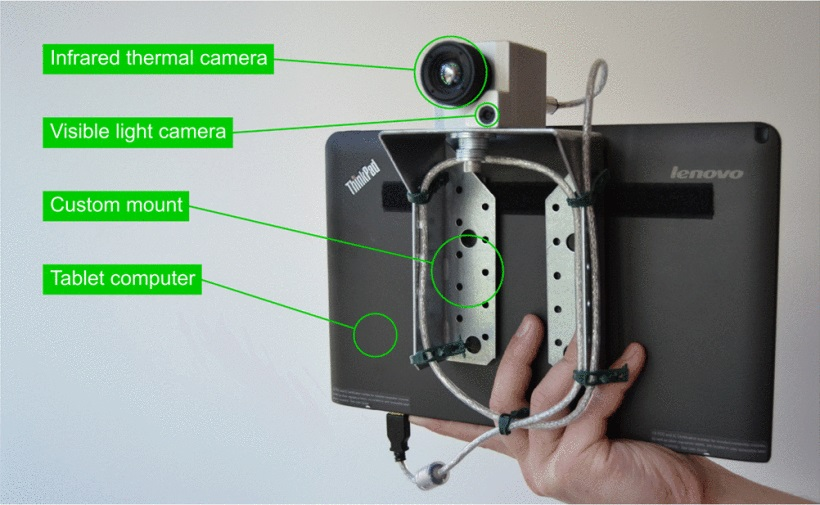
\includegraphics[width=8.5cm, height=5cm]{Hardware2}
	\caption{The hardware prototype used throughout Kurz's paper comprises a visible light camera and an infrared thermographic camera attached and connected to a tablet computer with a custom mount. \cite{Thermal}}
	\label{fig:hardware}
\end{figure}

\subsection{Hardware}
\label{Hardware}
The hardware in Kurz's \cite{Thermal} set up was a camera mounted to a tablet computer as shown in Figure \ref{fig:hardware}. It needed to be custom fitted since the technology for thermal imagery is not typically built into everyday devices, like tablets or phones. The camera on the tablet mixes a visible light camera, and a infrared camera in one package. The visible light camera is able to capture RGB images at 480x360 pixels and the infrared at 160x120 pixels. The parameters of the visible light camera and the infrared camera along with the 6DOF rigid body transformation from both cameras were calibrated. The calibration method Kurz used had a checkerboard pattern cut into bright cardboard, then attached to a warm dark surface like an LCD screen. This is done so that the visible light camera sees dark squares on a light surface, but the infrared camera sees light squares on a dark surface.


\subsection{Object Tracking}
\label{Object Tracking}
As mentioned above,  Kurz's goal is detecting touch in 3D space with real objects, which requires the ability to transform real objects relative to the camera. Metaio is a AR company that developed an object tracking software that can find the position and orientation of an object relative to the visible light camera in real time \cite{Thermal}. He used the Metaio software so that the visual light camera on the prototype was able to get the position and orientation of the object(s) used in the experiments.     

\begin{figure}
	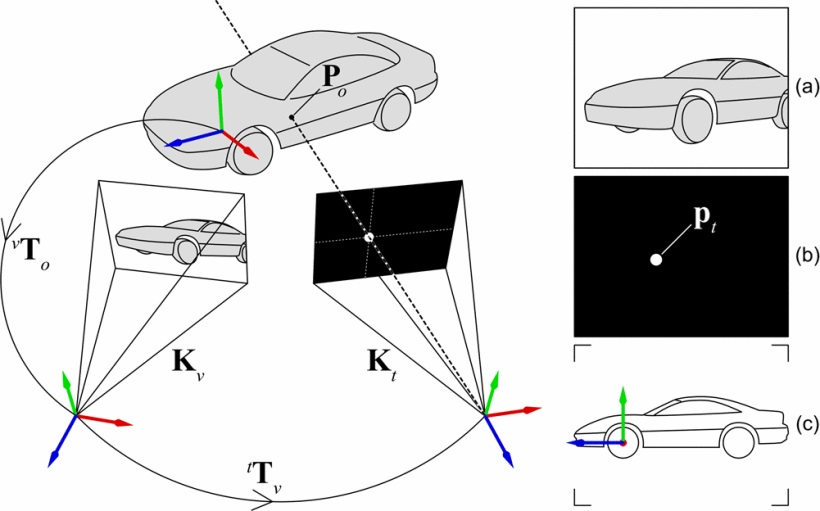
\includegraphics[width=8.5cm, height=7cm]{Tracking}
	\caption{Illustration of the involved coordinate systems and resources: a visible light camera image (a), a thermal camera image (b) and a model of the real object to interact with (c).\cite{Thermal}}
	\label{fig:Tracking}
\end{figure}

%\begin{figure}
%	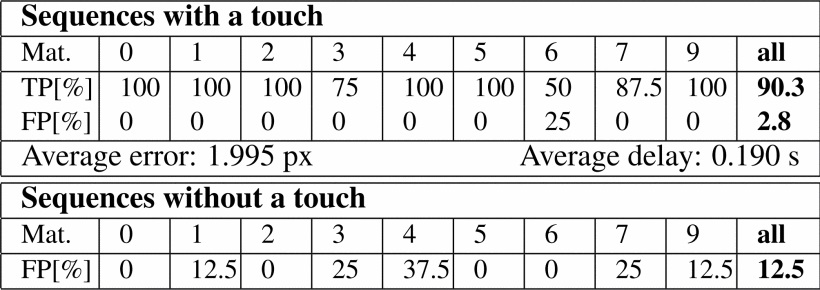
\includegraphics[width=8.5cm, height=3cm]{TouchData}
%	\caption{Evaluation results: true positive (TP) and false positive (FP) touch %detection on the test data set with different materials (mat.) \cite{Thermal}}
%	\label{fig:TouchData}
%\end{figure}


\subsection{Thermal Detection}
\label{Thermal Detection}
The two main obstacles that Kurz brings up is detecting the touch in thermal imaging, and being able to find where the touch occurred on a 3D object. First he explored temperature profiles of a surface being touched, obstructed, or not interacted with at all. The 4 cases of temperatures profiles are: Object-only, hand-only, obstruction-by-hand, and touch-by-hand. Object-only is just using the cameras to measure the relative constant temperature of an object. Hand only measured the temperature of a hand, expecting moderate temperature changes relative to fluctuating body temperature. Obstruction by hand starts with detecting an object and then having a hand come between the object and the camera, while not touching the object. The infrared will detect the rapid change from cool surface to a warm body, then rapidly back to the cool surface. Touch by hand is when the object is actually touched. The observed temperature  will start with the cool surface temperature and then rise when the warm body obstructs the area. Then once the hand moves away, instead of a rapid change back to a cool surface there is a rapid decrease to a temperature between that of the hand and the object. After this initial rapid decrease the area will slowly cool, reverting back to the starting temperature. 

Kurz used the OpenCV SimpleBlobDetector to calculate the size of the thermal fingerprints left on the object. Blobs are the set of circular areas returned by OpenCV's SimpleBlobDetector, they correspond to the touched area. Using a temperature range of \(t_1\) and \(t_2\) the thermal camera is able to detect if an object was touched. Below is how \(t_1\) and \(t_2\) are calculated

\(
\begin{matrix} \\
 t_{1}=(1-{1\over 16})t_{ min}+{1\over 16}t_{ max} & t_{2}=(1-{3\over 8})t_{ min}+{3\over 8}t_{ max}\cr 
 \end{matrix} \\\\
\)
This is calculated by taking \(t_{min}\) and \(t_{max}\), the minimum and maximum temperature recorded from the thermal camera, then applying those numbers to the SimpleBlobDetector. Along with knowing the temperature range to expect, an area range of \(a_{1}=0.32{\rm cm}^{2}\) and \(a_{2}=1.54{\rm cm}^{2}\) is used for detecting the blobs. the numbers used for \(a_{1}\) and \(a_{2}\) were determined by trial and error. Ignoring blobs with centers close to 10 pixels to the edge of the image, this is to reduce the amount of false positives from fingers entering and leaving the image. Kurz's experiments focused on single touch events, ignoring all blobs if there are multiple.

The touch position \(p_t\) is is the center of a detected blob in 2D space (see Figure \ref{fig:Tracking}(b)), this position needs to be transformed in order to find the 3D position \(P_o\) (see Figure \ref{fig:Tracking}). Taking \(p_t\) and using the Metaio software from above, one is able to find \(P_o\). Taking the visible light image \(K_v\) and a tracking model, an object tracker can find the 6DOF ridged body transformation \({^t}T_o\). Attaching that ridged body transformation to the calibrated transformation \({^t}T_v\) resulting in the position of the object to the thermal camera \(K_t\). This results in the device knowing the 3D position of the interaction in relation to both visible light and thermal cameras.
 
\begin{figure}
	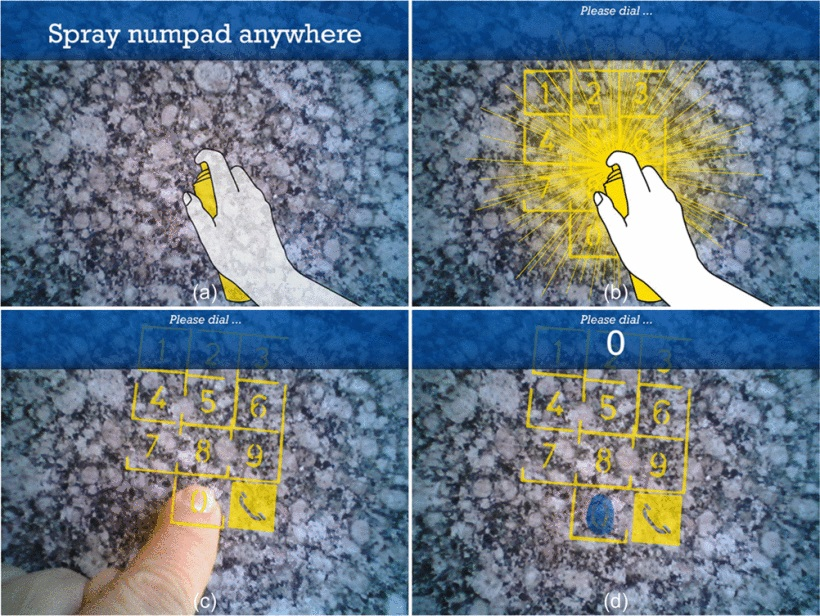
\includegraphics[width=8.5cm, height=8cm]{numpad}
	\caption{A number pad on a granite countertop seen through the screen of a mobile device \cite{Thermal}.}
	\label{fig:numpad}
\end{figure}

\begin{figure*}
	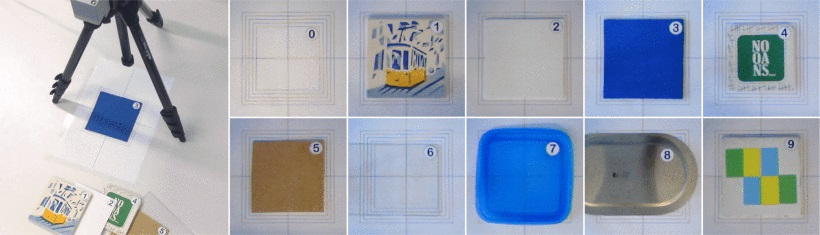
\includegraphics[width=18cm, height=5cm]{ThermalTesting}
	\caption{Different materials used in Kurz's evaluation: (0) paper on a plastic table-top, (1) ceramic, (2) rigid PVC, (3) foam plastic, (4) cardboard, (5) laminated fiber sheet, (6) glass, (7) thin plastic, (8) steel, (9) multi-layer board. \cite{Thermal}}
	\label{fig:ThermalTest}
\end{figure*}

\begin{figure}
	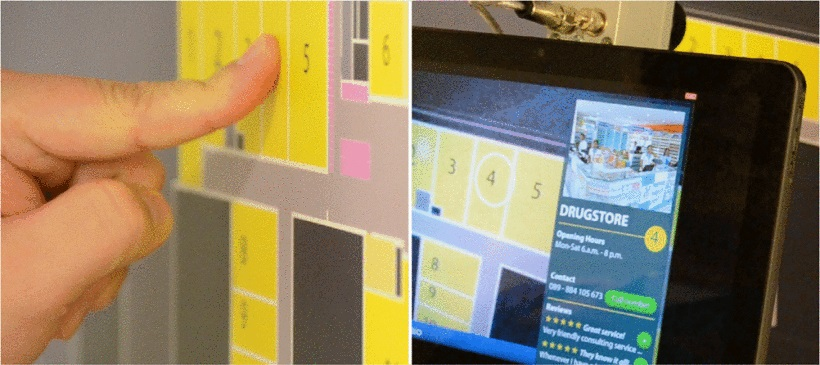
\includegraphics[width=8.5cm, height=6cm]{AugmentedFloorPlans}
	\caption{Interaction with a AR floor plan \cite{Thermal}.}
	\label{fig:FloorPlan}
\end{figure}

\subsection{Materials Tested}
\label{Materials Tested}
The blob detector is designed to handle objects that differ in material and temperature. This should also work for different users that have differing finger or body temperatures. The touch time and pressure would most likely be different form user to user. Kurz tested the algorithm with an array of materials one would encounter every day. the experiment consisted of different users touching different surfaces at different temperatures \cite{3D}. Figure \ref{fig:ThermalTest} is the testing environment Kurz used to test different materials. The materials tested are paper, plastics, glass, and metal, being placed on the table centered with the camera. The camera is positioned 300 mm above the materials being tested. The test involved four different people in a controlled office environment with ambient temperature at \(25^o\)C. 

A different group of four people did the same experiment, but outside in temperature of \(12^o\)C, leaving the test samples in the environment that they would be tested in for around thirty minutes to ensure they conformed to the environments temperature. The test consisted of having the person first pass their hand between the material and the camera, not touching the material. After that they were told just to touch the middle of the material as if it were a key on a keyboard. Notably it was not specified which finger to use and how to have the finger leave the object, leaving that entirely up to the subject. 

After this test was done Kurz had around 400 thermal images with a time stamp and labeled according to the action, material and testers name. The results of the tests showed that number 8, steel, from Figure \ref{fig:ThermalTest} does not work well with thermal interaction. This is due to the high rate at which steel dissipates heat, making it difficult to detect using their method. The data collected on steel was removed from test results, because of steels inability to retain heat. Out of the remaining 9 material sequences only two detected a touch in the wrong area, the rest detected touched areas correctly. Material 6, glass, from the outside tests had a false positives because the sticker appears warmer then the glass outdoors. 7 sequences could not detect touch due to the short period of contact. The false positives in the sequences without touch were quite high. This was attributed to residual heat left during the placement of the material under the camera.

\subsection{Applications}
\label{Thermal Applications}
Since the prototype from Figure \ref{fig:hardware} was a more of a hand held device, Kurz mentions that the thermal interaction could be possible with wearable technology, or head-mounted displays. A common example of wearable technology would be a smart watch, and for head-mounted displays it is Google Glass. If this method is applied to wearable technology, or head-mounted displays, it would be a solution for interacting with technology without a touchscreen.     

Two of the main applications mentioned in the paper are Spray-On GUIs, Graphical User Interface, and augmented floor plans. A Spray-On GUIs utilize any surface available to the user, an example would be a number pad on a granite countertop (see Figure \ref{fig:numpad}). Using the camera of the mobile device this application superimposes a virtual number pad onto a surface. in reality, the GUI is not on the actual surface, but is visible via the screen of the mobile device. Using the screen as a reference the user can dial numbers by pressing the location. Once sprayed on the GUI location is fixed in one place Kurz called it instance tracking, which creates an image and can track it. Spray-On GUIs need a fixed location, because mobile devices lack stability when held in ones hand. The camera can move around freely and the object remains in one place. Otherwise, the user could try and dial seven, but the camera could move to the left and then seven turns into eight. When one of the keys is touched, the camera is able to determine the corresponding key that was touched based on the location in the thermal image. 

The AR floor plan is used when there is a printed floor plan of a building, for example a mall. The AR floor plan allows a user to press his/her desired location on the floor plan while pointed the mobile device at the map. Detecting this interaction with the map the device is able to make a query and tell what store or restaurant is at the pressed location. It is also able to display other information such as business hours, ratings, website link, and contact information. With this approach there would be no need for Spray-on GUI since the camera would use the shapes of the floor plan in lieu of virtual buttons. This type of method would work best for interfaces that users regular access to. The floor plan of a mall is the prime example of AR floor plans, but if a user had to find a dial pad sticker when they needed to make a call, that would be less appealing to users.      


\section{3D Data Visualization with SAR}
\label{sec:3D Data Visualization}
I will now focus on a paper that explores the use of SAR as a tool for 3D data visualization \cite{3D}. As mentioned in Section \ref{sec:Spatial Augmented Reality}, SAR uses projectors to augment what is already there. Data visualization is the representation of data thought the use of images. Thomas et al. focus more on 3D data visualization, and not manipulation \cite{3D}. Being able to see and touch the data is their main focus, because using multiple senses can help the user remember the data being displayed. They define their proposed use of SAR as a tool for 3D visualization in following ways. First they propose the use of SAR to benefit the user's ability to see, understand, and manipulate 3D visualization data. Second is the tabletop SAR prototype (see Figure \ref{fig:Tabletop}). Some of the uses would include visualizing charts, maps, or graphs. The projections on the physical object define areas of investigation in a 3D volume, more will be disused in Section \ref{sec:3D Applications}. Third is the large applications of SAR, called \textit{CAVE} which is discussed later as well.

\subsection{Visualizing Data}
\label{sec:Visualizing Data}
Some basic examples would be pie charts, scatter-plots, and bar charts, ect. Data visualization can be used in any field, from showing the demographics of a neighborhood to displaying how many shooting stars happen over the course of a year, or even weather maps. Visualizing data with though pictures is an effective way to show someone information quickly and efficiently. Humans tend to recall and process pictures more easily than words, that is part of why humans have so many ways to display date.   

\subsection{Applications}
\label{sec:3D Applications}
Thomas et al. \cite{3D} mention two ways that 3D data visualization can be applied in the real world. The main one they mention is the tabletop. This is a proposed system where there is a 2D display (they call it a fish tank view), a table with the physical object(s), the virtual volume, the hand held pointing device, 6DOF trackers, and the projectors (see Figure \ref{fig:Tabletop}). A large display is used to provide detailed views of the date being visualized, providing a reference to where the user is in the 3D volume. The virtual volume is the space around the table-top, starting from the surface of the table extending up a foot or two. In the virtual volume a user could zoom in, or out, on the data being visualized on the physical object using the hand held device. An example this action would be displaying the weather maps of North America, then zooming in on the north west region, or zoom out to displaying more of the world. The physical object is what the projectors are using to visualize the 3D data. As mentioned the hand held device is used in the virtual volume, but it is tracked by the 6DOF trackers to track where the user is in the room.

The second method is the CAVE system, Marner et al. \cite{CAVE} states
\begin{quote}
	The virtual environment (VE) closest to SAR is probably the CAVE (Cave Automatic Virtual Environment). Both SAR and CAVE systems employ projectors as the primary display technology. \cite{CAVE}
\end{quote}
SAR systems will project onto the object of interest; whereas in a CAVE the object being projected onto becomes a window to the virtual world, making the area of focus on the data instead of the object itself. Thomas et al. \cite{3D} used the CAVE system as a large scale version of the tabletop method. CAVE systems require more space than the table-top method this is due to the need for more 6DOF tracers and projectors for the setup to work. Other then that, how the user interacts with CAVE in no different then the table-top system. The scale of the CAVE system requires many wall, this is what would be projected on by the projectors as the large display. The physical objects and virtual volume would be larger. As illustrated in Figure \ref{fig:Cave} the physical objects are larger than the small cone from the table-top method. The benefit the CAVE model is being able to increase the number of collaborators/viewers. Figure \ref{fig:Cave} is one of a couple CAVE configurations possible with this technology. Other configurations just change the shape and size of the system. The CAVE would be a better choice, over the table-top method, if the needs required more collaborators, or the need to display the visual date to a larger audience. 

\begin{figure}
	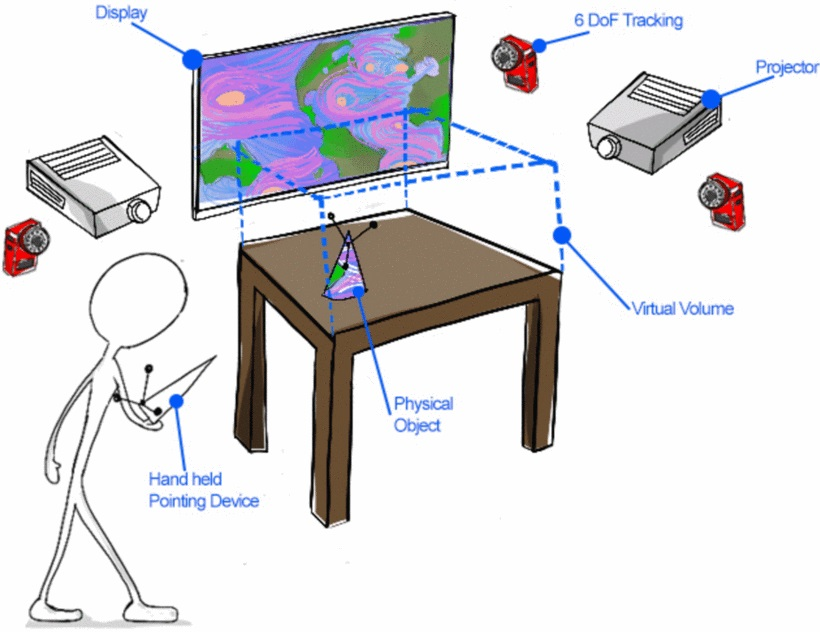
\includegraphics[width=8.5cm, height=5cm]{Tabletop}
	\caption{the tabletop set up that Thomas et al. propose \cite{3D}}
	\label{fig:Tabletop}
\end{figure}

\subsection{Limitations}
\label{sec:Limitations}
The initial experimentation with Thomas et al.'s \cite{3D} prototype showed a number of limitations. The first is that the lighting the room must be controlled, as details in the gradients of the projected data may be lost with too much ambient lighting. Like anything projector-related, it works best in dim-to-dark rooms, depending on the type of projector. and would require upgrading to a more powerful projector.

\subsection{Conclusion}
\label{sec:Conclusion}
The goal of Thomas et al. \cite{3D} was presenting SAR as a tool to enrich the process of 3D visualization. They laid out their plan on using SAR with these three goals. They start by explaining the benefit to the user's abilities to interpret and retain the data being presented. The second goal was the implementation of the table-top they proposed. Letting the user manipulate the data by zooming in or out, the user handles the data, improving retention of the information. Lastly, increasing the possible applications of visualizing 3D data with SAR by proposing the CAVE system. The CAVE would allow more people to view the data being displayed at one time.

\begin{figure}
	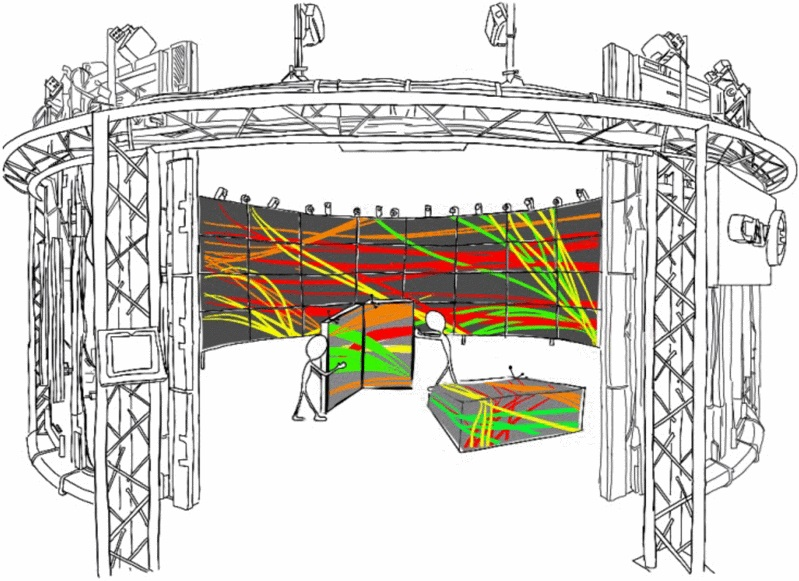
\includegraphics[width=8.5cm, height=5cm]{Cave}
	\caption{One of the CAVE systems mentioned by Thomas et al. \cite{3D}}
	\label{fig:Cave}
\end{figure}  

\section{Combining Thermal Interaction + 3D Visualization}
\label{sec:Joining Together}
Both Sections \ref{sec:Thermal Interaction} and \ref{sec:3D Data Visualization} talk about different ideas. Section \ref{sec:Thermal Interaction} talks about using thermal heat signatures to detect interaction in AR, where Section \ref{sec:3D Data Visualization} discuses using SAR as a tool to visualize data. This section will discus how they will work together. In Section \ref{sec:3D Data Visualization}, a 6DOF object is needed to track ones position, but with the thermal interactions the camera is able to detect positions of objects using visible light cameras. Knowing the position and orientation of the object one can find the position and orientation of the person looking at it.   

\subsection{Applications}
\label{Applications}
Some possible applications of this kind of combination could be in education and transportation. With education the proposed idea would be for a class to wear head-mounted displays containing a visible light camera and a thermal camera, like the camera from Figure \ref{fig:hardware}, but smaller. Also, each of the students' desks would essentially become the table-top system mentioned in Figure \ref{fig:Tabletop} with a physical object, a sphere will be the physical object being projected onto. The lesson in this example is geography, the sphere on each students desk has the map of the world being displayed onto its surface. The teacher would have control over the zooming in and out aspect, unless the teacher wanted the class to explore the maps to ask or answer questions.

Transportation would benefit from the ability to detect where a user wants to go and then display the information pertaining to route and time the train, bus, or other forms of public transit. Using the AR floor plan system, from section \ref{Thermal Applications}, in the form of a train or bus route a system could detect someone wants to take a bus to the local store. In turn the projector would highlight where the closest bus on the route is, and if the user would have to take multiple buses to reach the destination. 


\section{Conclusion}
\label{Conclusion}
This section will highlight some of the strengths and weaknesses of both the methods in Sections \ref{sec:Thermal Interaction} and \ref{sec:3D Data Visualization}. Starting with Section \ref{sec:Thermal Interaction} moving towards using AR more in everyday life could lead to ethical problem. Heimo et al. \cite{ethics} mentions that in an age where government surveillance is almost everywhere, an increase in AR technology could lead from the current way surveillance is conducted to a more self surveillance type of system.
As mentioned above education and transportation are just a few areas that would benefit from the union of these technologies. Working together to combine strengths they reduce the weaknesses the methods had prior, but also they will share the weaknesses that were not taken care of.  


\section{Acknowledgments}
\label{sec:Acknowledgments}
I would like to take this time to thank my advisor Nic McPhee, co-teacher Elena Machkasova    , Ian Buck, and everyone who gave feedback to help refine this paper. 
\bibliographystyle{abbrv}
\bibliography{annotatedBibliography}

\end{document}